\documentclass{standalone}
\usepackage{tikz}
\usetikzlibrary{patterns, positioning}


\begin{document}
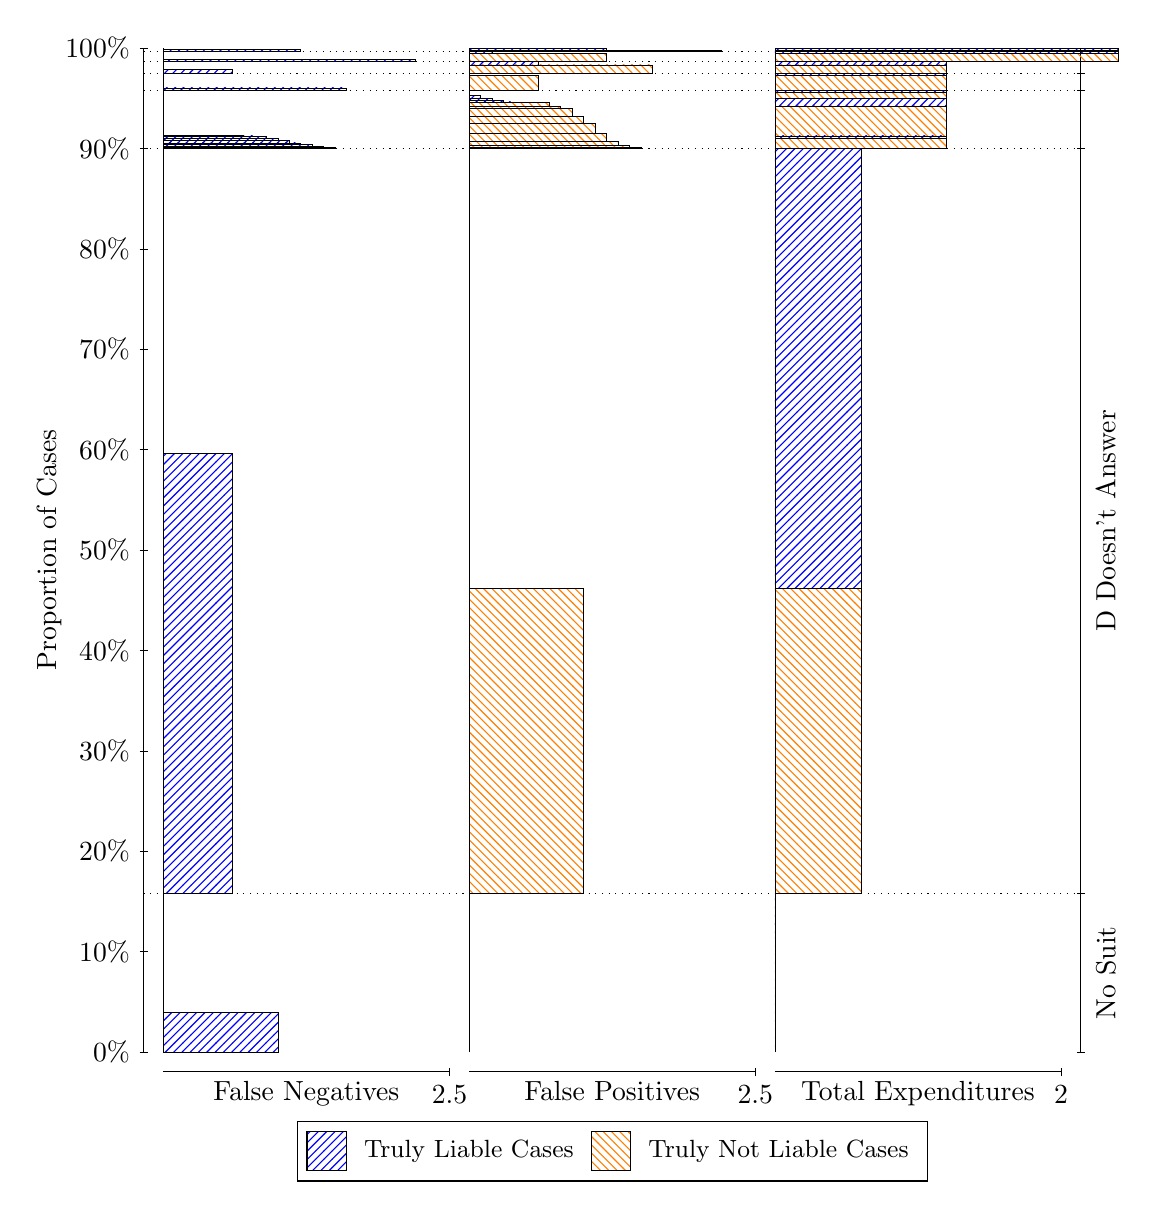
\begin{tikzpicture}
\draw[black, very thin] (1.5,1.75) -- (1.5,14.5);
\node[rotate=90, text=black, anchor=center] at (0.3, 8.125) {Proportion of Cases};
\draw[black, very thin] (1.45,1.75) -- (1.55,1.75);
\node[text=black, anchor=east] at (1.45, 1.75) {0\%};
\draw[black, very thin] (1.45,3.025) -- (1.55,3.025);
\node[text=black, anchor=east] at (1.45, 3.025) {10\%};
\draw[black, very thin] (1.45,4.3) -- (1.55,4.3);
\node[text=black, anchor=east] at (1.45, 4.3) {20\%};
\draw[black, very thin] (1.45,5.575) -- (1.55,5.575);
\node[text=black, anchor=east] at (1.45, 5.575) {30\%};
\draw[black, very thin] (1.45,6.85) -- (1.55,6.85);
\node[text=black, anchor=east] at (1.45, 6.85) {40\%};
\draw[black, very thin] (1.45,8.125) -- (1.55,8.125);
\node[text=black, anchor=east] at (1.45, 8.125) {50\%};
\draw[black, very thin] (1.45,9.4) -- (1.55,9.4);
\node[text=black, anchor=east] at (1.45, 9.4) {60\%};
\draw[black, very thin] (1.45,10.675) -- (1.55,10.675);
\node[text=black, anchor=east] at (1.45, 10.675) {70\%};
\draw[black, very thin] (1.45,11.95) -- (1.55,11.95);
\node[text=black, anchor=east] at (1.45, 11.95) {80\%};
\draw[black, very thin] (1.45,13.225) -- (1.55,13.225);
\node[text=black, anchor=east] at (1.45, 13.225) {90\%};
\draw[black, very thin] (1.45,14.5) -- (1.55,14.5);
\node[text=black, anchor=east] at (1.45, 14.5) {100\%};

\draw[black, very thin] (13.4,1.75) -- (13.4,14.5);
\draw[black, very thin] (13.35,1.75) -- (13.45,1.75);
\node[anchor=west] at (13.35, 1.75) {};
\draw[black, very thin] (13.35,3.7622) -- (13.45,3.7622);
\node[anchor=west] at (13.35, 3.7622) {};
\draw[black, very thin] (13.35,13.226) -- (13.45,13.226);
\node[anchor=west] at (13.35, 13.226) {};
\draw[black, very thin] (13.35,13.966) -- (13.45,13.966);
\node[anchor=west] at (13.35, 13.966) {};
\draw[black, very thin] (13.35,14.181) -- (13.45,14.181);
\node[anchor=west] at (13.35, 14.181) {};
\draw[black, very thin] (13.35,14.332) -- (13.45,14.332);
\node[anchor=west] at (13.35, 14.332) {};
\draw[black, very thin] (13.35,14.454) -- (13.45,14.454);
\node[anchor=west] at (13.35, 14.454) {};
\draw[black, very thin] (13.35,14.5) -- (13.45,14.5);
\node[anchor=west] at (13.35, 14.5) {};

\draw[black, very thin, pattern color=blue, pattern=north east lines] (1.75,1.75) rectangle (3.2033,2.2539);
\draw[black, very thin, pattern color=orange, pattern=north west lines] (1.75,2.2539) rectangle (1.75,3.7622);
\draw[black, very thin, pattern color=blue, pattern=north east lines] (1.75,3.7622) rectangle (2.622,9.3516);
\draw[black, very thin, pattern color=orange, pattern=north west lines] (1.75,9.3516) rectangle (1.75,13.226);
\draw[black, very thin, pattern color=blue, pattern=north east lines] (1.75,13.226) rectangle (3.93,13.24);
\draw[black, very thin, pattern color=blue, pattern=north east lines] (1.75,13.24) rectangle (3.7847,13.249);
\draw[black, very thin, pattern color=blue, pattern=north east lines] (1.75,13.249) rectangle (3.6393,13.273);
\draw[black, very thin, pattern color=blue, pattern=north east lines] (1.75,13.273) rectangle (3.494,13.294);
\draw[black, very thin, pattern color=blue, pattern=north east lines] (1.75,13.294) rectangle (3.3487,13.327);
\draw[black, very thin, pattern color=blue, pattern=north east lines] (1.75,13.327) rectangle (3.2033,13.353);
\draw[black, very thin, pattern color=blue, pattern=north east lines] (1.75,13.353) rectangle (3.058,13.375);
\draw[black, very thin, pattern color=blue, pattern=north east lines] (1.75,13.375) rectangle (2.9127,13.384);
\draw[black, very thin, pattern color=blue, pattern=north east lines] (1.75,13.384) rectangle (2.7673,13.387);
\draw[black, very thin, pattern color=orange, pattern=north west lines] (1.75,13.387) rectangle (1.75,13.966);
\draw[black, very thin, pattern color=blue, pattern=north east lines] (1.75,13.966) rectangle (4.0753,13.995);
\draw[black, very thin, pattern color=orange, pattern=north west lines] (1.75,13.995) rectangle (1.75,14.181);
\draw[black, very thin, pattern color=blue, pattern=north east lines] (1.75,14.181) rectangle (2.622,14.226);
\draw[black, very thin, pattern color=orange, pattern=north west lines] (1.75,14.226) rectangle (1.75,14.332);
\draw[black, very thin, pattern color=blue, pattern=north east lines] (1.75,14.332) rectangle (4.9473,14.352);
\draw[black, very thin, pattern color=orange, pattern=north west lines] (1.75,14.352) rectangle (1.75,14.454);
\draw[black, very thin, pattern color=blue, pattern=north east lines] (1.75,14.454) rectangle (3.494,14.48);
\draw[black, very thin, pattern color=orange, pattern=north west lines] (1.75,14.48) rectangle (1.75,14.5);
\draw[black, very thin, pattern color=orange, pattern=north west lines] (5.6333,1.75) rectangle (5.6333,3.2584);
\draw[black, very thin, pattern color=blue, pattern=north east lines] (5.6333,3.2584) rectangle (5.6333,3.7622);
\draw[black, very thin, pattern color=orange, pattern=north west lines] (5.6333,3.7622) rectangle (7.0867,7.6363);
\draw[black, very thin, pattern color=blue, pattern=north east lines] (5.6333,7.6363) rectangle (5.6333,13.226);
\draw[black, very thin, pattern color=orange, pattern=north west lines] (5.6333,13.226) rectangle (7.8133,13.241);
\draw[black, very thin, pattern color=orange, pattern=north west lines] (5.6333,13.241) rectangle (7.668,13.26);
\draw[black, very thin, pattern color=orange, pattern=north west lines] (5.6333,13.26) rectangle (7.5227,13.315);
\draw[black, very thin, pattern color=orange, pattern=north west lines] (5.6333,13.315) rectangle (7.3773,13.416);
\draw[black, very thin, pattern color=orange, pattern=north west lines] (5.6333,13.416) rectangle (7.232,13.541);
\draw[black, very thin, pattern color=orange, pattern=north west lines] (5.6333,13.541) rectangle (7.0867,13.63);
\draw[black, very thin, pattern color=orange, pattern=north west lines] (5.6333,13.63) rectangle (6.9413,13.732);
\draw[black, very thin, pattern color=orange, pattern=north west lines] (5.6333,13.732) rectangle (6.796,13.759);
\draw[black, very thin, pattern color=orange, pattern=north west lines] (5.6333,13.759) rectangle (6.6507,13.805);
\draw[black, very thin, pattern color=blue, pattern=north east lines] (5.6333,13.805) rectangle (6.36,13.808);
\draw[black, very thin, pattern color=blue, pattern=north east lines] (5.6333,13.808) rectangle (6.2147,13.817);
\draw[black, very thin, pattern color=blue, pattern=north east lines] (5.6333,13.817) rectangle (6.0693,13.839);
\draw[black, very thin, pattern color=blue, pattern=north east lines] (5.6333,13.839) rectangle (5.924,13.865);
\draw[black, very thin, pattern color=blue, pattern=north east lines] (5.6333,13.865) rectangle (5.7787,13.898);
\draw[black, very thin, pattern color=blue, pattern=north east lines] (5.6333,13.898) rectangle (5.6333,13.966);
\draw[black, very thin, pattern color=orange, pattern=north west lines] (5.6333,13.966) rectangle (6.5053,14.152);
\draw[black, very thin, pattern color=blue, pattern=north east lines] (5.6333,14.152) rectangle (5.6333,14.181);
\draw[black, very thin, pattern color=orange, pattern=north west lines] (5.6333,14.181) rectangle (7.9587,14.287);
\draw[black, very thin, pattern color=blue, pattern=north east lines] (5.6333,14.287) rectangle (6.5053,14.332);
\draw[black, very thin, pattern color=orange, pattern=north west lines] (5.6333,14.332) rectangle (7.3773,14.434);
\draw[black, very thin, pattern color=blue, pattern=north east lines] (5.6333,14.434) rectangle (5.924,14.454);
\draw[black, very thin, pattern color=orange, pattern=north west lines] (5.6333,14.454) rectangle (8.8307,14.474);
\draw[black, very thin, pattern color=blue, pattern=north east lines] (5.6333,14.474) rectangle (7.3773,14.5);
\draw[black, very thin, pattern color=orange, pattern=north west lines] (9.5167,1.75) rectangle (9.5167,3.2584);
\draw[black, very thin, pattern color=blue, pattern=north east lines] (9.5167,3.2584) rectangle (9.5167,3.7622);
\draw[black, very thin, pattern color=orange, pattern=north west lines] (9.5167,3.7622) rectangle (10.607,7.6363);
\draw[black, very thin, pattern color=blue, pattern=north east lines] (9.5167,7.6363) rectangle (10.607,13.226);
\draw[black, very thin, pattern color=orange, pattern=north west lines] (9.5167,13.226) rectangle (11.697,13.351);
\draw[black, very thin, pattern color=blue, pattern=north east lines] (9.5167,13.351) rectangle (11.697,13.384);
\draw[black, very thin, pattern color=orange, pattern=north west lines] (9.5167,13.384) rectangle (11.697,13.765);
\draw[black, very thin, pattern color=blue, pattern=north east lines] (9.5167,13.765) rectangle (11.697,13.862);
\draw[black, very thin, pattern color=orange, pattern=north west lines] (9.5167,13.862) rectangle (11.697,13.936);
\draw[black, very thin, pattern color=blue, pattern=north east lines] (9.5167,13.936) rectangle (11.697,13.966);
\draw[black, very thin, pattern color=orange, pattern=north west lines] (9.5167,13.966) rectangle (11.697,14.152);
\draw[black, very thin, pattern color=blue, pattern=north east lines] (9.5167,14.152) rectangle (11.697,14.181);
\draw[black, very thin, pattern color=orange, pattern=north west lines] (9.5167,14.181) rectangle (11.697,14.287);
\draw[black, very thin, pattern color=blue, pattern=north east lines] (9.5167,14.287) rectangle (11.697,14.332);
\draw[black, very thin, pattern color=orange, pattern=north west lines] (9.5167,14.332) rectangle (13.877,14.434);
\draw[black, very thin, pattern color=blue, pattern=north east lines] (9.5167,14.434) rectangle (13.877,14.454);
\draw[black, very thin, pattern color=orange, pattern=north west lines] (9.5167,14.454) rectangle (13.877,14.474);
\draw[black, very thin, pattern color=blue, pattern=north east lines] (9.5167,14.474) rectangle (13.877,14.5);
\draw[black, dotted] (1.5,3.7622) -- (13.4,3.7622);
\draw[black, dotted] (1.5,13.226) -- (13.4,13.226);
\draw[black, dotted] (1.5,13.966) -- (13.4,13.966);
\draw[black, dotted] (1.5,14.181) -- (13.4,14.181);
\draw[black, dotted] (1.5,14.332) -- (13.4,14.332);
\draw[black, dotted] (1.5,14.454) -- (13.4,14.454);
\draw[black, very thin] (1.75,1.5) -- (5.3833,1.5);
\node[text=black, anchor=north] at (3.5667, 1.5) {False Negatives};
\draw[black, very thin] (5.3833,1.45) -- (5.3833,1.55);
\node[text=black, anchor=north] at (5.3833, 1.45) {2.5};

\draw[black, very thin] (5.6333,1.5) -- (9.2667,1.5);
\node[text=black, anchor=north] at (7.45, 1.5) {False Positives};
\draw[black, very thin] (9.2667,1.45) -- (9.2667,1.55);
\node[text=black, anchor=north] at (9.2667, 1.45) {2.5};

\draw[black, very thin] (9.5167,1.5) -- (13.15,1.5);
\node[text=black, anchor=north] at (11.333, 1.5) {Total Expenditures};
\draw[black, very thin] (13.15,1.45) -- (13.15,1.55);
\node[text=black, anchor=north] at (13.15, 1.45) {2};

\node[text=black, centered, rotate=90] at (13.72, 2.7561) {No Suit};
\node[text=black, centered, rotate=90] at (13.72, 8.494) {D Doesn't Answer};






\draw (7.449999999999999,1.5) node[draw=none] (baseCoordinate) {};
\begin{scope}[align=center]
        \matrix[scale=0.5, draw=black, below=0.5cm of baseCoordinate, nodes={draw}, column sep=0.1cm]{
            \node[rectangle, draw, minimum width=0.5cm, minimum height=0.5cm, pattern color=blue, pattern=north east lines] {}; &
            \node[draw=none, font=\small, text=black] (B) {Truly Liable Cases}; &
            \node[rectangle, draw, minimum width=0.5cm, minimum height=0.5cm, pattern color=orange, pattern=north west lines] {}; &
            \node[draw=none, font=\small, text=black] (B) {Truly Not Liable Cases}; \\
            };
\end{scope}

\end{tikzpicture}
\end{document}